\documentclass[answers]{exam}
\input{global}
\input{problem-sets}
\usepackage{fontawesome5}

\setrandomizerseed{1}

\header{{Name:\enspace\makebox[6cm]{\hrulefill}}\\Physics}{}{Test on Unit 10: Mechanical Waves}
\runningheader{Physics}{}{Test on Unit 10: Mechanical Waves}


\begin{document}

\noindent \textbf{Questions \ref{9V4n3}--\ref{VhYcC}.} The figure below shows a wave.

\begin{center}
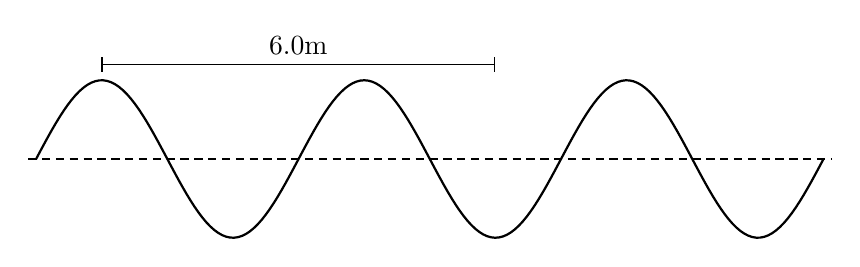
\begin{tikzpicture}[x=1cm]
    \draw[densely dashed] (-0.1,0) -- (10.1,0);
    \draw[thick,domain=0:10,samples=200] plot(\x,{sin(deg(2*pi*\x/(10/3)))});
    \draw[shift={(0,0.2)},|-|] (0.83,1) -- (5.83,1) node[above,pos=0.5] {\SI{6.0}{m}};
\end{tikzpicture}
\end{center}

\begin{questions}
\question \label{9V4n3}
What is the wavelength of this wave?

\begin{randomizechoices}
    \correctchoice \SI{4.0}{m}
    \choice \SI{2.0}{m}
    \choice \SI{8.0}{m}
    \choice \SI{16.0}{m}  
\end{randomizechoices}



\question \label{VhYcC}
If the frequency of the wave from is 2.0 hertz, what is the speed of the wave?

\begin{randomizechoices}
    \correctchoice \SI{8.0}{m/s}
    \choice \SI{4.0}{m/s}
    \choice \SI{16.0}{m/s}
    \choice \SI{2.0}{m/s}
\end{randomizechoices}

\question
Two wave pulses of equal amplitude are moving towards each other on a string, as shown in the figure below.


\begin{center}
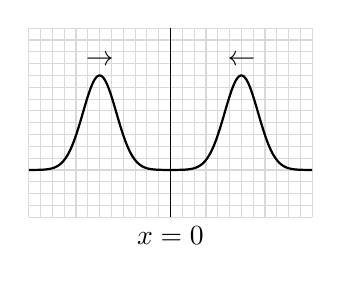
\begin{tikzpicture}[y=3mm,x=3mm]
    \draw[step=0.5,black!15] (-6,-2) grid (6,6);
    \draw[domain=-6:0,samples=120,thick] plot (\x,{4*exp(-(\x+3)^2)});
    \node[above] at (-3,4) {$\rightarrow$};
    \draw[domain=0:6,samples=120,thick] plot (\x,{4*exp(-(\x-3)^2)});
    \node[above] at (+3,4) {$\leftarrow$};
    \draw (0,6) -- (0,-2) node[below] {$x=0$};
\end{tikzpicture}
\end{center}

Which of the following graphs represents how the string will appear when the pulses meet at $x=0$?


\begin{EnvUplevel}
\centering
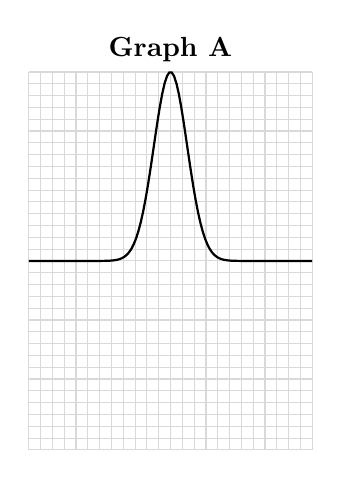
\begin{tikzpicture}[y=3mm,x=3mm]
    \draw[step=0.5,black!15] (-6,-8) grid (6,8);
    \draw[domain=-6:6,samples=120,thick] plot (\x,{4*exp(-(\x)^2) + 4*exp(-(\x)^2)});
    \node[above] at (current bounding box.north) {\textbf{Graph A}};
\end{tikzpicture}
\hspace{2mm}
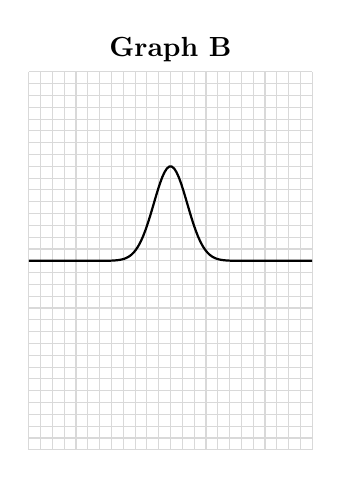
\begin{tikzpicture}[y=3mm,x=3mm]
    \draw[step=0.5,black!15] (-6,-8) grid (6,8);
    \draw[domain=-6:6,samples=120,thick] plot (\x,{2*exp(-(\x)^2) + 2*exp(-(\x)^2)});
    \node[above] at (current bounding box.north) {\textbf{Graph B}};
\end{tikzpicture}
\hspace{2mm}
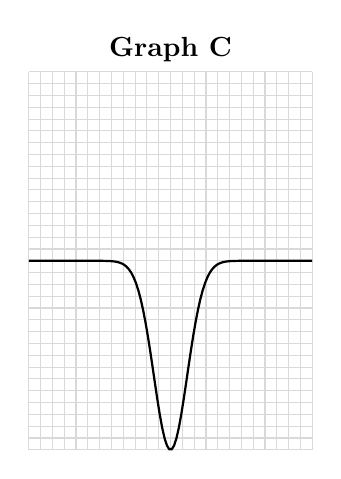
\begin{tikzpicture}[y=3mm,x=3mm]
    \draw[step=0.5,black!15] (-6,-8) grid (6,8);
    \draw[domain=-6:6,samples=120,thick] plot (\x,{-4*exp(-(\x)^2) - 4*exp(-(\x)^2)});
    \node[above] at (current bounding box.north) {\textbf{Graph C}};
\end{tikzpicture}
\hspace{2mm}
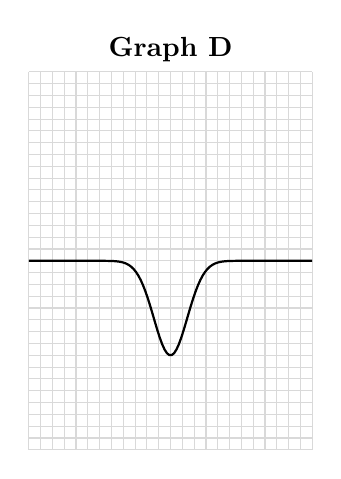
\begin{tikzpicture}[y=3mm,x=3mm]
    \draw[step=0.5,black!15] (-6,-8) grid (6,8);
    \draw[domain=-6:6,samples=120,thick] plot (\x,{-2*exp(-(\x)^2) - 2*exp(-(\x)^2)});
    \node[above] at (current bounding box.north) {\textbf{Graph D}};
\end{tikzpicture}
\end{EnvUplevel}

\begin{randomizeoneparchoices}[norandomize]
    \correctchoice Graph A
    \choice Graph B
    \choice Graph C
    \choice Graph D
\end{randomizeoneparchoices}


\clearpage 

\question
Two wave pulses with unequal amplitudes are moving towards each other on a string, as shown in the figure below.


\begin{center}
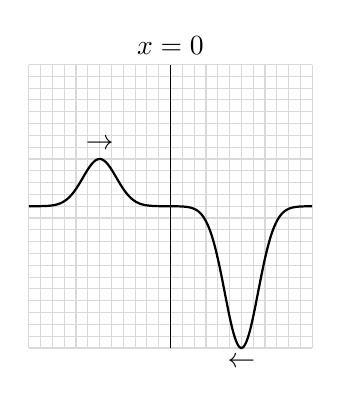
\begin{tikzpicture}[y=3mm,x=3mm]
    \draw[step=0.5,black!15] (-6,-6) grid (6,6);
    \draw[domain=-6:0,samples=120,thick] plot (\x,{2*exp(-(\x+3)^2)});
    \node[above] at (-3,2) {$\rightarrow$};
    \draw[domain=0:6,samples=120,thick] plot (\x,{-6*exp(-(\x-3)^2)});
    \node[below] at (+3,-6) {$\leftarrow$};
    \draw (0,6) -- (0,-6) node[above,pos=0] {$x=0$};
\end{tikzpicture}
\end{center}

Which of the following graphs represents how the string will appear when the pulses meet at $x=0$?


\begin{EnvUplevel}
\centering
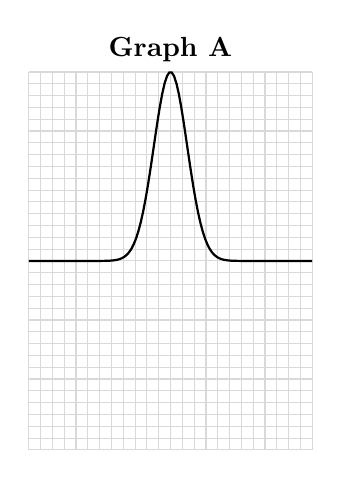
\begin{tikzpicture}[y=3mm,x=3mm]
    \draw[step=0.5,black!15] (-6,-8) grid (6,8);
    \draw[domain=-6:6,samples=120,thick] plot (\x,{4*exp(-(\x)^2) + 4*exp(-(\x)^2)});
    \node[above] at (current bounding box.north) {\textbf{Graph A}};
\end{tikzpicture}
\hspace{2mm}
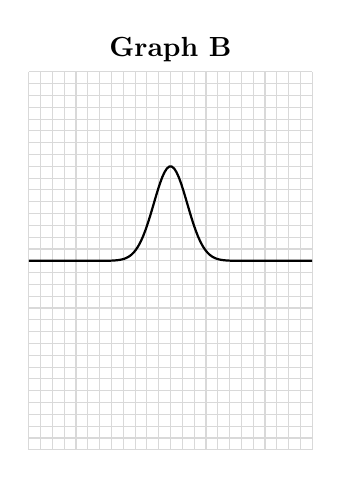
\begin{tikzpicture}[y=3mm,x=3mm]
    \draw[step=0.5,black!15] (-6,-8) grid (6,8);
    \draw[domain=-6:6,samples=120,thick] plot (\x,{2*exp(-(\x)^2) + 2*exp(-(\x)^2)});
    \node[above] at (current bounding box.north) {\textbf{Graph B}};
\end{tikzpicture}
\hspace{2mm}
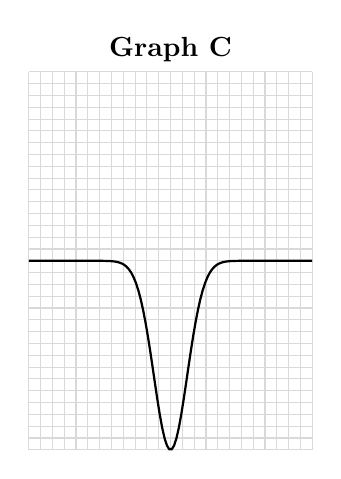
\begin{tikzpicture}[y=3mm,x=3mm]
    \draw[step=0.5,black!15] (-6,-8) grid (6,8);
    \draw[domain=-6:6,samples=120,thick] plot (\x,{-4*exp(-(\x)^2) - 4*exp(-(\x)^2)});
    \node[above] at (current bounding box.north) {\textbf{Graph C}};
\end{tikzpicture}
\hspace{2mm}
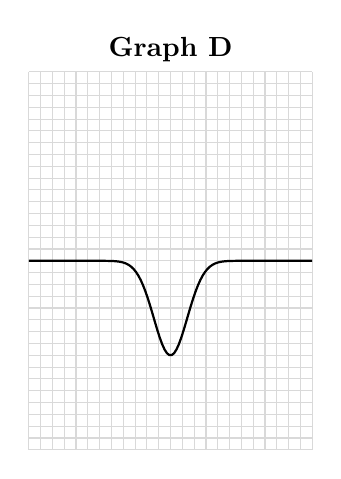
\begin{tikzpicture}[y=3mm,x=3mm]
    \draw[step=0.5,black!15] (-6,-8) grid (6,8);
    \draw[domain=-6:6,samples=120,thick] plot (\x,{2*exp(-(\x)^2) - 6*exp(-(\x)^2)});
    \node[above] at (current bounding box.north) {\textbf{Graph D}};
\end{tikzpicture}
\end{EnvUplevel}

\begin{randomizeoneparchoices}[norandomize]
    \choice Graph A
    \choice Graph B
    \choice Graph C
    \correctchoice Graph D
\end{randomizeoneparchoices}

\question
Sound is a \fillin[longitudinal][4cm]\ wave.

\begin{randomizechoices}
    \correctchoice longitudinal
    \choice transverse
    \choice electromagnetic
    \choice seismic
\end{randomizechoices}

\question
The figure below shows particles of air as a sound wave propagates through them. 

\begin{center}
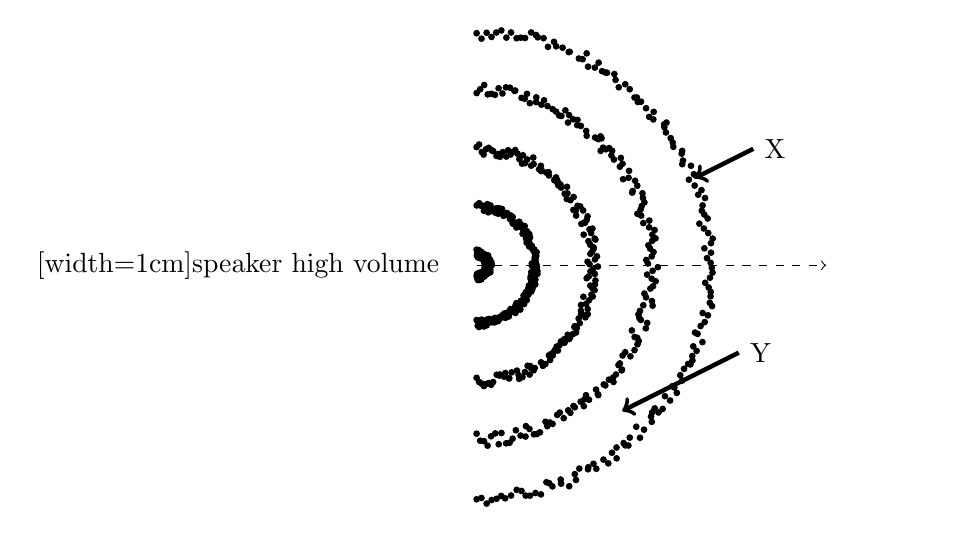
\begin{tikzpicture}
    \begin{axis}[height=7.5cm,width=7.5cm,
      cycle list={
        only marks,mark size=1pt\\
        only marks,mark size=1pt\\
      },
      xmin=0,xmax=8,
      ymin=-4,ymax=4,
      domain=270:360+90,
      samples=150,
      axis line style={draw=none},
      ticks=none,
      clip=false,
    ]
    \draw[dashed,->] (0,0) -- (6,0);
    \addplot ({(0.2+0.07*rand)*cos(x)},{(0.2+0.07*rand)*sin(x)});
    \addplot ({(1.0+0.07*rand)*cos(x)},{(1.0+0.07*rand)*sin(x)});
    \addplot ({(2.0+0.10*rand)*cos(x)},{(2.0+0.10*rand)*sin(x)});
    \addplot ({(3.0+0.12*rand)*cos(x)},{(3.0+0.12*rand)*sin(x)});
    \addplot ({(4.0+0.12*rand)*cos(x)},{(4.0+0.12*rand)*sin(x)});
    
    \draw[<-,ultra thick] (3.75,1.5) -- ++(axis direction cs: 1,0.5) node[right] {X};
    \draw[<-,ultra thick] (2.5,-2.5) -- ++(axis direction cs: 2,1) node[right] {Y};
    
    \node[left=1em] at (0,0) {\twemoji[width=1cm]{speaker high volume}};
    \end{axis}
\end{tikzpicture}
\end{center}

Region X is called a \fillin[compression][4cm], and Region Y is a \fillin[rarefaction][4cm].

\begin{randomizechoices}
    \correctchoice compression; \hspace{1mm} rarefaction
    \choice rarefaction; \hspace{1mm} compression
    \choice wavelength; \hspace{1mm} frequency
    \choice frequency; \hspace{1mm} wavelength
\end{randomizechoices}


\question
Students are using an oscilloscope to analyze two musical notes, X and Y. The graphs below represent the data recorded.

\begin{EnvUplevel}
\centering
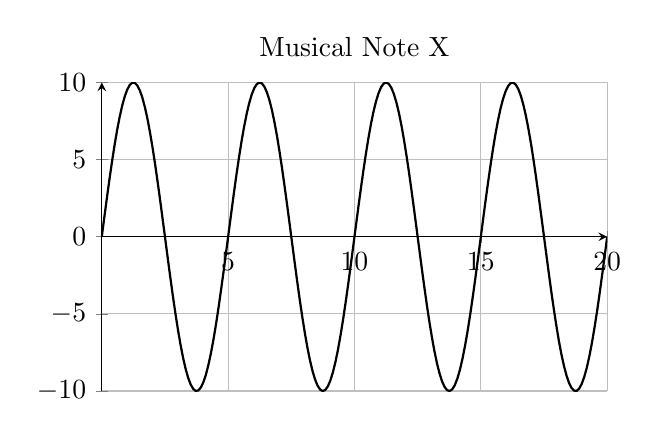
\begin{tikzpicture}
    \begin{axis}[width=8cm,height=5.5cm,
        % ylabel={Volts (V)},
        % xlabel={Time (s)},
        axis y line=left,
        axis x line=center,
        ymin=-10,ymax=10,
        xmin=0,xmax=20,
        ytick={-10,-5,...,10},
        xtick={0,5,...,20},
        grid=both,
        title={Musical Note X}
    ]
        \addplot[thick,domain=0:20,samples=200] {10*sin(deg(2*pi*x/(20/4)))};
    \end{axis}
\end{tikzpicture}
\hspace{5mm}
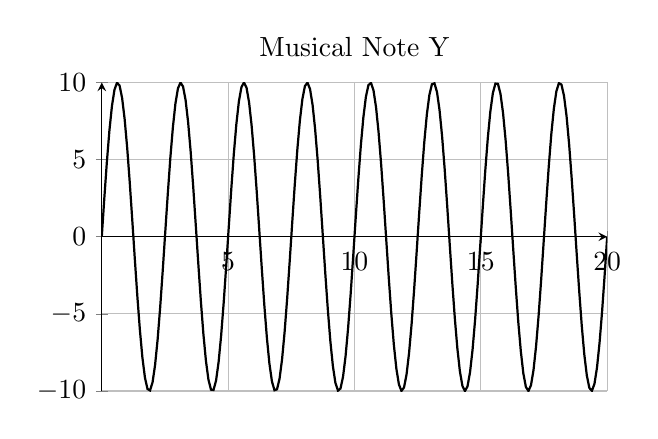
\begin{tikzpicture}
    \begin{axis}[width=8cm,height=5.5cm,
        % ylabel={Volts (V)},
        % xlabel={Time (s)},
        axis y line=left,
        axis x line=center,
        ymin=-10,ymax=10,
        xmin=0,xmax=20,
        ytick={-10,-5,...,10},
        xtick={0,5,...,20},
        grid=both,
        title={Musical Note Y}
    ]
        \addplot[thick,domain=0:20,samples=200] {10*sin(deg(2*pi*x/(20/8)))};
    \end{axis}
\end{tikzpicture}
\end{EnvUplevel}

The two notes have the same\ldots 

\begin{randomizechoices}
    \choice wavelengths
    \choice frequencies
    \correctchoice amplitudes
    \choice periods
\end{randomizechoices}

% \question
% Sam has incorrectly labeled the wave diagram shown.

% \begin{center}
% \begin{tikzpicture}[y=1.2cm,x=8mm]
%     \draw[densely dashed] (0,0) -- (10,0);
%     \draw[thick,domain=0:10,samples=200] plot(\x,{sin(deg(2*pi*\x/(10/2)))});
%     \draw[|-|] (-0.2,-1) -- (-0.2,1) node[left,pos=0.5] {$A$};
%     \draw[densely dashed] (0,1) -- (1.25,1) (0,-1) -- (3.75,-1);
%     \draw[|-|] (5,1.1) -- (10,1.1) node[above,pos=0.5] {$\lambda$};
%     \draw[densely dashed] (5,1) -- (5,0) (10,1) -- (10,0);
% \end{tikzpicture}
% \end{center}

% Which of the following are true regarding Sam's labels in the wave diagram?
% Select \textbf{TWO} correct answers.

% \begin{randomizechoices}
%     \correctchoice The wavelength is correctly labeled.
%     \choice The wavelength is only half of what is shown by the label.
%     \choice The amplitude is correctly labeled.
%     \correctchoice The amplitude is only half of what is shown by the label.
%     \choice The amplitude and wavelength labels are reversed.
% \end{randomizechoices}

\question 
Wave P and wave Q are similar waves that are being compared. If the frequency in wave Q doubles, and both waves travel at the same speed, how would the wavelength change?

\begin{randomizechoices}
    \choice Wave Q's wavelength would be cut by a fourth.
    \choice Wave Q's wavelength would be multiplied by a factor of four.
    \correctchoice Wave Q's wavelength would be cut in half.
    \choice Wave Q's wavelength would be doubled.
\end{randomizechoices}

\question
In physics lab, the class measures the speed of sound and obtained an average value of \SI{347}{m/s}. The teacher then asks students if all sound frequencies travel at the same speed in air. Which student gives the best answer?

\begin{randomizechoices}
    \choice No, drum sounds are low frequency and travel faster because you can hear them from farther away.
    \choice No, if the class had used longer wave lengths and the same frequency, the answer would have been twice as great, as shown by the equation $v = f \lambda$ .
    \correctchoice Yes, band instruments have different frequencies, yet you hear their\\sounds together.
    \choice Yes, I remember that velocity value was used in a movie about breaking the time barrier.
\end{randomizechoices}

% \question
% Two speakers, $S_1$ and $S_2$, operating in phase in the same medium produce the circular wave patterns shown in the diagram below.

% \begin{center}
% \begin{tikzpicture}
%     \fill (-1,0) circle (0.05);
%     \fill (+1,0) circle (0.05);
%     \draw[thick] (-2,0) arc (180:0:1);
%     \draw[thick] (+2,0) arc (0:180:1);
%     \draw[thick] (-2,0) arc (180:0:3);
%     \draw[thick] (+2,0) arc (0:180:3);
%     \draw[densely dashed] (-1,0) arc (180:0:2);
%     \draw[densely dashed] (+1,0) arc (0:180:2);
%     \draw[densely dashed] (-5,0) arc (180:0:4);
%     \draw[densely dashed] (+5,0) arc (0:180:4);
%     \draw[fill=white] (0,3.9) circle (0.25) node {A};
%     \draw[fill=white] (-1.75,2.9) circle (0.25) node {B};
%     \draw[fill=white] (0,2.85) circle (0.25) node {C};
%     \draw[fill=white] (+1.75,2.9) circle (0.25) node {D};
%     \draw[fill=white] (-1.25,2) circle (0.25) node {E};
%     \draw[fill=white] (+1.25,2) circle (0.25) node {F};
% \end{tikzpicture}
% \end{center}

% At which points is constructive interference occurring?

% \begin{randomizechoices}[norandomize]
%     \correctchoice Point A
%     \choice Point B
%     \correctchoice Point C
%     \choice Point D
%     \choice Point E
%     \choice Point F
% \end{randomizechoices}

\ifprintanswers \else \clearpage \fi

\question
Based on the image, where would an observer perceive the fire truck to have a \underline{higher} pitch than what its siren sounds like when stationary?

\begin{center}
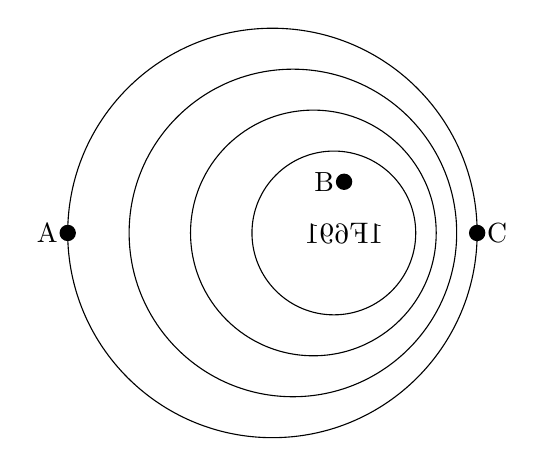
\begin{tikzpicture}[x=1.3cm,y=1.3cm]
    % \draw (-5,0) node {\Strichmaxerl[3]} node[above=4mm] {Alice};
    % \draw (+5,0) node {\Strichmaxerl[3]} node[above=4mm] {Bob};
    \node at (0,0) {\reflectbox{\resizebox{1cm}{!}{\usym{1F691}}}}; 
    \draw (-0.10,0) circle (0.8);
    \draw (-0.30,0) circle (1.2);
    \draw (-0.50,0) circle (1.6);
    \draw (-0.70,0) circle (2.0);
    \fill (-2.7,0) circle (0.08) node[left=0.1] {A};
    \fill (0,0.5) circle (0.08) node[left=0.1] {B};
    \fill (1.3,0) circle (0.08) node[right=0.1] {C};
\end{tikzpicture}
\end{center}


\begin{randomizechoices}[norandomize]
    \choice Behind the fire truck, at position A.
    \choice Next to the fire truck, at position B.
    \correctchoice In front of the fire truck, at position C.
    \choice They would all hear the same pitch.
\end{randomizechoices}

\question
A musical instrument plays a note which causes a glass in the room to emit a similar tone by itself. Which of the following explains this phenomenon?
Select \textbf{TWO} correct answers.

\begin{randomizechoices}
    \choice The glass will emit a tone when any frequency sound is present.
    \correctchoice The glass produces a tone when a specific frequency sound is present.
    \correctchoice Resonance causes the glass to emit a similar tone.
    \choice Reflection causes the glass to emit a similar tone.
    \choice Interference causes the glass to emit a similar tone.
\end{randomizechoices}

\question
Based on the image, where would an observer perceive the fire truck to have a \underline{lower} pitch than what its siren sounds like when stationary?

\begin{center}
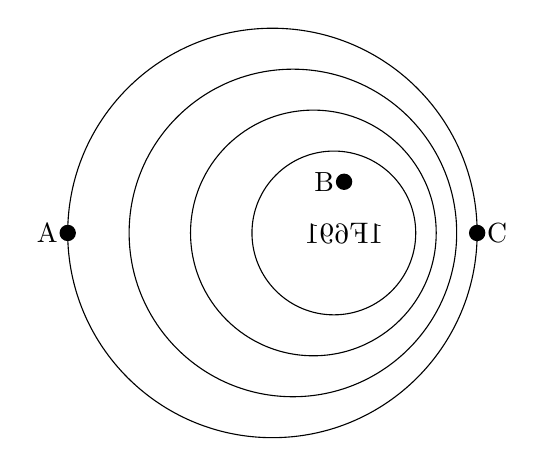
\begin{tikzpicture}[x=1.3cm,y=1.3cm]
    % \draw (-5,0) node {\Strichmaxerl[3]} node[above=4mm] {Alice};
    % \draw (+5,0) node {\Strichmaxerl[3]} node[above=4mm] {Bob};
    \node at (0,0) {\reflectbox{\resizebox{1cm}{!}{\usym{1F691}}}}; 
    \draw (-0.10,0) circle (0.8);
    \draw (-0.30,0) circle (1.2);
    \draw (-0.50,0) circle (1.6);
    \draw (-0.70,0) circle (2.0);
    \fill (-2.7,0) circle (0.08) node[left=0.1] {A};
    \fill (0,0.5) circle (0.08) node[left=0.1] {B};
    \fill (1.3,0) circle (0.08) node[right=0.1] {C};
\end{tikzpicture}
\end{center}


\begin{randomizechoices}[norandomize]
    \correctchoice Behind the fire truck, at position A.
    \choice Next to the fire truck, at position B.
    \choice In front of the fire truck, at position C.
    \choice They would all hear the same pitch.
\end{randomizechoices}


\begin{EnvUplevel}
    \textbf{Question \ref{YdeyW}.} Two pulses, A and B, travel toward each other along the same rope, as shown in the diagram.
    
\begin{center}
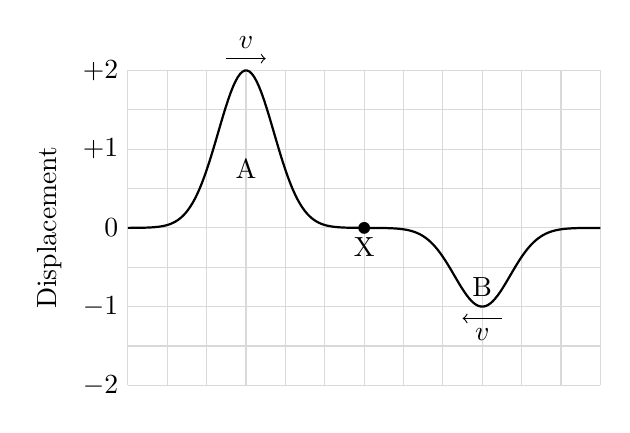
\begin{tikzpicture}[x=5mm,y=5mm]
    \draw[step=1,black!15] (-6,-4) grid (6,4);
    \fill (0,0) circle (0.15) node[below=0.15] {X};
    \draw[thick,domain=-6:0,samples=100,thick] plot (\x,{4*exp(-(\x+3)^2)});
    \draw[thick,domain=0:+6,samples=100,thick] plot (\x,{-2*exp(-(\x-3)^2)});
    \draw[->] (-3.5,4.3) -- (-2.5,4.3) node[above,pos=0.5] {$v$};
    \draw[->] (3.5,-2.3) -- (2.5,-2.3) node[below,pos=0.5] {$v$};
    \node at (-3,1.5) {A};
    \node at (+3,-1.5) {B};
    \node[left] at (-6,+4) {$+2$};
    \node[left] at (-6,+2) {$+1$};
    \node[left] at (-6,+0) {$0$};
    \node[left] at (-6,-2) {$-1$};
    \node[left] at (-6,-4) {$-2$};
    \node[rotate=90] at (-8,0) {Displacement};
\end{tikzpicture}
\end{center}
\end{EnvUplevel}

\question \label{YdeyW}
What will be the vertical displacement of the rope when the two pulses meet at X?

\begin{randomizechoices}[norandomize]
    \choice $-2$ units
    \choice $-1$ units
    \choice $0$ units
    \correctchoice $+1$ units
    \choice $+2$ units
\end{randomizechoices}

% \question \label{P5iOs}
% Which of the following statements about this scenario shown in the diagram are correct?
% Choose TWO correct answers.

% \begin{randomizechoices}
%     \choice There is constructive interference.
%     \correctchoice There is destructive interference.
%     \choice The Doppler Effect occurs.
%     \correctchoice The speed of the pulses remains constant.
%     \choice The speed of the pulses changes.
% \end{randomizechoices}

\question
A Love wave, one of the four types of waves associated with earthquakes, is a transverse wave in which the surface of Earth moves back and forth as the wave passes. What is the speed of a Love wave that has a period of \SI{150}{s} and a wavelength of \SI{620}{km}?

\begin{randomizechoices}
    \choice \SI{9.3e4}{km/s}
    \correctchoice \SI{4.1}{km/s}
    \choice \SI{470}{km/s}
    \choice \SI{9.3}{km/s}
\end{randomizechoices}

% \ifprintanswers \else \clearpage \fi

% \question
% A mass, $M$, is hung from a spring attached to a fixed point X, and reaches equilibrium at position B. The mass is then raised to position A and released. The mass oscillates between positions A and C.

% \begin{center}
% \begin{tikzpicture}
%     \draw[decorate,decoration={coil,segment length=3.5pt,post length=2mm,pre length=2mm,amplitude=2.5mm}] (0,0) -- (0,-3) node[below,pos=0,shift={(0.45,0.05)}] {X};
%     \draw[fill=black!15] (-0.3,-3) rectangle (0.3,-3.6) node[pos=0.5] {$M$}; 
%     \draw[densely dashed] (0.5,-1.8) -- (2.5,-1.8) node[right] {A};
%     \draw[densely dashed] (0.5,-3.3) -- (2.5,-3.3) node[right] {B};
%     \draw[densely dashed] (0.5,-4.8) -- (2.5,-4.8) node[right] {C};
%     \draw[fill=lightgray] (-1,0.1) -- (-1,0) -- (1,0) -- (1,0.1);
% \end{tikzpicture}
% \end{center}

% Which position shows where the mass will have its highest elastic potential energy?
% Select ONE correct answer.

% \begin{randomizechoices}[norandomize]
%     \choice Position A
%     \choice Position B
%     \choice Position C
%     \choice Position X
% \end{randomizechoices}

\question
An oscillating object, like a swing, transforms energy back and forth between which two storage banks?

\begin{randomizechoices}
    \choice Thermal energy and nuclear energy.
    \correctchoice Potential energy (gravitational or elastic) and kinetic energy.
    \choice Chemical energy and electrical energy.
    \choice Sound energy and light energy.
\end{randomizechoices}

\question
A student uses a rope tied to a wall and forms a standing wave, as shown in Figure 1.


\begin{EnvUplevel}
\centering
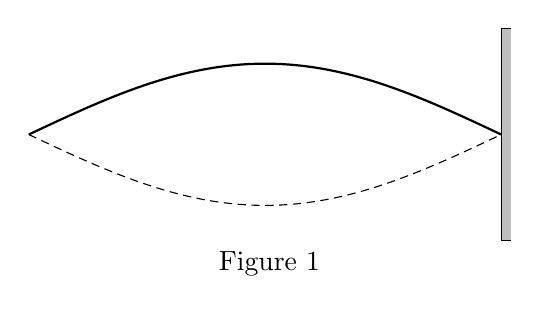
\begin{tikzpicture}[x=6mm,y=9mm]
    \draw[thick,domain=0:10,samples=100] plot({\x},{sin(deg(2*pi*\x/(10/0.5)))});
    \draw[densely dashed,domain=0:10,samples=100] plot({\x},{-sin(deg(2*pi*\x/(10/0.5)))});
    \draw[fill=lightgray] (10.2,1.5) -- (10,1.5) -- (10,-1.5) -- (10.2,-1.5);
    \node[below] at (current bounding box.south) {Figure 1};
\end{tikzpicture}
\hspace{2cm}
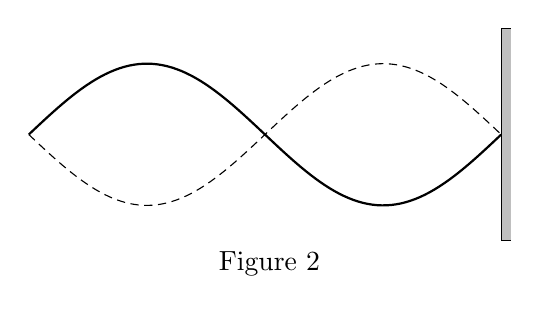
\begin{tikzpicture}[x=6mm,y=9mm]
    \draw[thick,domain=0:10,samples=100] plot({\x},{sin(deg(2*pi*\x/(10/1.0)))});
    \draw[densely dashed,domain=0:10,samples=100] plot({\x},{-sin(deg(2*pi*\x/(10/1.0)))});
    \draw[fill=lightgray] (10.2,1.5) -- (10,1.5) -- (10,-1.5) -- (10.2,-1.5);
    \node[below] at (current bounding box.south) {Figure 2};
\end{tikzpicture}
\end{EnvUplevel}

The student then produces the second standing wave, as shown in Figure 2. Which of the following wave properties increases?

\begin{randomizechoices}
    \choice amplitude
    \correctchoice frequency
    \choice period
    \choice wavelength
\end{randomizechoices}

% \ifprintanswers \else \clearpage \fi

% \question
% The diagram below represents a standing wave produced in a string by a vibrating wave generator. 


% \begin{center}
% \begin{tikzpicture}[rotate around={-90:(0,0)},x=5mm,y=5mm]
%     \draw[ultra thick] (0,-1) -- (0,1) node[pos=0.5,above,align=center] {\small supporting\\ \small rod};
%     \draw[thick,domain=0:10,samples=100] plot({\x},{sin(deg(2*pi*\x/(10/1.5)))});
%     \draw[densely dashed,domain=0:10,samples=100] plot({\x},{-sin(deg(2*pi*\x/(10/1.5)))});
%     \draw[->] (0.25,-4) -- (0.25,-2) node[left,pos=0] {Segment A};
%     {\ifprintanswers \color{red} \fi \draw[->] (1.67,-4) -- (1.67,-2) node[left,pos=0] {Segment B};}
%     \draw[->] (3.33,-4) -- (3.33,-2) node[left,pos=0] {Segment C};
%     {\ifprintanswers \color{red} \fi \draw[->] (5.00,-4) -- (5.00,-2) node[left,pos=0] {Segment D};}
%     \draw[->] (6.67,-4) -- (6.67,-2) node[left,pos=0] {Segment E};
%     {\ifprintanswers \color{red} \fi \draw[->] (8.33,-4) -- (8.33,-2) node[left,pos=0] {Segment F};}
%     \draw[->] (10.0,-4) -- (10.0,-2) node[left,pos=0] {Segment G};
%     \draw (10.3,0) node {\faEthernet} node[shift={(3,0)}] {\small wave generator};
% \end{tikzpicture}
% \end{center}

% Which segments in the standing wave would be considered antinodes?

% \begin{randomizechoices}[norandomize]
%     \choice Segment A
%     \correctchoice Segment B
%     \choice Segment C
%     \correctchoice Segment D
%     \choice Segment E
%     \correctchoice Segment F
%     \choice Segment G
% \end{randomizechoices}

\question
A wave is diffracted as it passes through an opening in a barrier. Which of the following determines the amount of diffraction that the wave undergoes as it passes through the opening? Select TWO correct answers.

\begin{randomizechoices}
    \choice the amplitude of the wave
    \choice the speed of the wave
    \correctchoice the wavelength of the wave
    \choice the distance of the barrier from the wave source
    \correctchoice the size of the opening
\end{randomizechoices}

% \question
% The bending of a wave when it crosses from one medium to another is called

% \begin{randomizechoices}
%     \choice interference
%     \choice diffraction
%     \choice reflection
%     \correctchoice refraction
% \end{randomizechoices}

% \ifprintanswers \else \clearpage \fi


\question
An upward wave pulse travels along a rope toward a boundary.

\begin{center}
\begin{tikzpicture}[x=8mm,y=1.2cm]
    \draw[thick,domain=-3:2.85,samples=100] plot (\x,{exp(-(\x)^2)});
    \draw (3,1) -- (3,-1);
    \draw (2.85,0) arc (180:540:0.15 and 0.05);
    \draw[->] (-0.5,1.2) -- (0.5,1.2);
\end{tikzpicture}
\end{center}

If the end of the rope is attached to a ring that can slide freely up and down a pole (a free end), how will the pulse reflect?

\begin{EnvUplevel}
\centering
\begin{tikzpicture}[x=6mm,y=9mm]
    {\ifprintanswers \color{red} \fi
    \draw[thick,domain=-3:2.85,samples=100] plot (\x,{exp(-(\x)^2)});
    \draw (3,1) -- (3,-1);
    \draw (2.85,0) arc (180:540:0.15 and 0.05);
    \draw[->] (0.5,1.2) -- (-0.5,1.2);
    \node[above=5mm] at (current bounding box.north) {Pulse A};
    }
\end{tikzpicture}
\hspace{1cm}
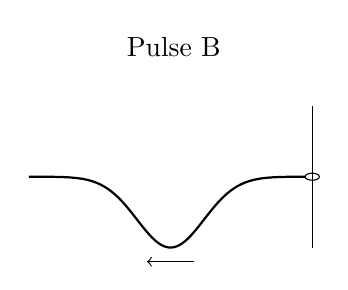
\begin{tikzpicture}[x=6mm,y=9mm]
    \draw[thick,domain=-3:2.85,samples=100] plot (\x,{-exp(-(\x)^2)});
    \draw (3,1) -- (3,-1);
    \draw (2.85,0) arc (180:540:0.15 and 0.05);
    \draw[->] (0.5,-1.2) -- (-0.5,-1.2);
    \node[above=5mm] at (current bounding box.north) {Pulse B};
\end{tikzpicture}
\hspace{1cm}
\begin{tikzpicture}[x=6mm,y=9mm]
    \draw[thick,domain=-3:2.85,samples=100] plot (\x,0);
    \draw (3,1) -- (3,-1);
    \draw (2.85,0) arc (180:540:0.15 and 0.05);
    \node[above=5mm] at (current bounding box.north) {Pulse C};
\end{tikzpicture}
\end{EnvUplevel}

\begin{randomizechoices}[norandomize]
    \correctchoice Pulse A
    \choice Pulse B
    \choice Pulse C
\end{randomizechoices}


\begin{EnvUplevel}
\textbf{Questions \ref{Q1}--\ref{Q2}.} The figure below shows the displacement from equilibrium for a wave on a string as a function of position.

\begin{center}
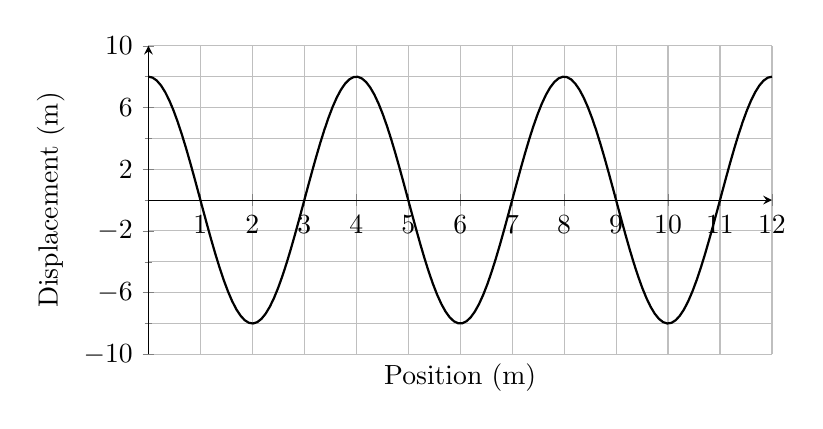
\begin{tikzpicture}
    \begin{axis}[height=5.5cm,
        width=9.5cm,
        axis y line=left,
        axis x line=center,
        ylabel={Displacement (m)},
        xlabel={Position (m)},
        x label style={at={(axis description cs: 0.5,0)},below},
        ymin=-10,ymax=10,
        xmin=0,xmax=12,
        ytick={-10,-6,...,10},
        xtick={0,1,...,12},
        grid=both,
        clip=false,
        minor y tick num=1,
        ]
        \addplot[thick,domain=0:12,samples=150] {8*cos(deg(2*pi*x/4)};
    \end{axis}
\end{tikzpicture}
\end{center}
\end{EnvUplevel}



\question \label{Q1}
What is the wave's amplitude?

\begin{randomizechoices}
    \correctchoice \SI{8}{m}
    \choice \SI{16}{m}
    \choice \SI{4}{m}
    \choice \SI{2}{m}
\end{randomizechoices}

\question \label{Q2}
The wavelength of the wave is

\begin{randomizechoices}
    \choice \SI{8}{m}
    \choice \SI{16}{m}
    \correctchoice \SI{4}{m}
    \choice \SI{2}{m}
\end{randomizechoices}

\question
What wave property is being measured in the figure below?

\begin{center}
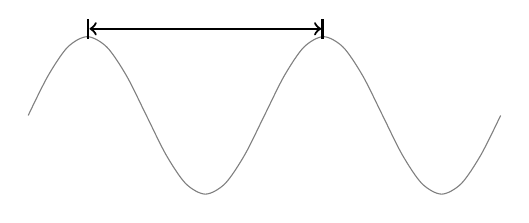
\begin{tikzpicture}[y=1cm,x=3cm]
    \draw[gray,domain=0:2,smooth] plot(\x,{sin(deg(2*pi*\x))});
    \draw[thick,|<->|,yshift=1mm] (0.25,1) -- ++(1,0);
\end{tikzpicture}
\end{center}

\begin{randomizechoices}
    \correctchoice wavelength
    \choice amplitude
    \choice frequency
    \choice wave speed
\end{randomizechoices}

\question
What wave characteristic is being measured in the figure below?

\begin{center}
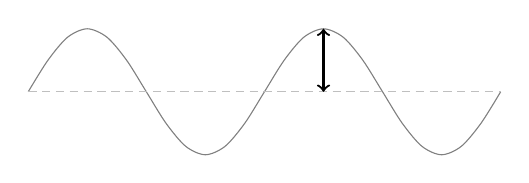
\begin{tikzpicture}[y=0.8cm,x=3cm]
    \draw[gray,domain=0:2,smooth] plot(\x,{sin(deg(2*pi*\x))});
    \draw[lightgray,densely dashed] (0,0) -- (2,0);
    \draw[thick,<->] (1.25,0) -- ++(0,1);
\end{tikzpicture}
\end{center}

\begin{randomizechoices}
    \choice wavelength
    \correctchoice amplitude
    \choice frequency
    \choice wave speed
\end{randomizechoices}

\question 
The transverse wave shown in the figure below is produced by disturbing one end a coil at a rate of \SI{3}{Hz}. Find the wave speed.

\begin{center}
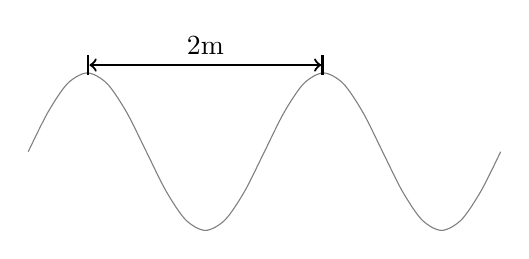
\begin{tikzpicture}[y=1cm,x=3cm]
    \draw[gray,domain=0:2,smooth] plot(\x,{sin(deg(2*pi*\x))});
    \draw[thick,|<->|,yshift=1mm] (0.25,1) -- ++(1,0) node[above,pos=0.5] {\SI{2}{m}};
\end{tikzpicture}
\end{center}

\ifprintanswers
{\color{red}
$v = f\lambda$
}
\fi

\begin{randomizechoices}[keeplast]
    \correctchoice \SI{6}{m/s}
    \choice \SI{5}{m/s}
    \choice \SI{3}{m/s}
    \choice \SI{2}{m/s}
    \choice More information is needed.
\end{randomizechoices}

\clearpage

\question 
As a pendulum swings back and forth, it completes 30 cycles in one minute.

\begin{center}
%%%...Tikzpicture inspired by Boas (Mathematical Physics) pg. 344)
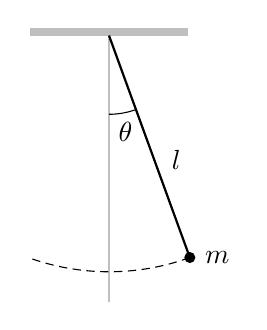
\begin{tikzpicture}
    \draw[lightgray] (-1,0) -- (1,0) (0,0) -- (0,{-3.5*sin(75)});
    \fill[lightgray] (-1,0) rectangle (1,0.1);
    \coordinate (P) at ({3*cos(70)},{-3*sin(70)});
    \draw[thick] (0,0) -- (P) node[pos=0.65,above right] {$l$};
    \fill (P) circle (2pt) node[right=2pt] {$m$};
    \draw (0,-1) arc (270:290:1) node[below,pos=0.6] {$\theta$};
    \draw[densely dashed] (P) arc (290:250:3);
\end{tikzpicture}
\end{center}

What is the period of oscillation?

\ifprintanswers
{\color{red}

$T = \frac{\text{total time}}{\text{\# cycles}} = \frac{\SI{60}{s}}{\SI{30}{cycles}} = \boxed{\SI{2.0}{s}}$

\medskip
}
\fi

\begin{randomizechoices}
    \choice 30 seconds
    \correctchoice 2 seconds
    \choice 1/30 seconds
    \choice 0.5 seconds
\end{randomizechoices}

\question
A group of students conducts an experiment using a long coil to study the properties of waves.

\begin{center}
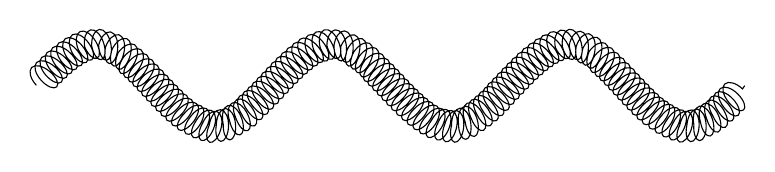
\begin{tikzpicture}
    \draw[decorate,decoration={coil,
        segment length=2.5pt,
        amplitude=2mm
        },domain=0:3,x=3cm,y=5mm,samples=150] plot(\x,{sin(deg(2*pi*\x))});
\end{tikzpicture}
\end{center}

After taking multiple sets of data, they produce the graph shown below and conclude that wavelength is inversely proportional to some measured property of the wave.

\begin{center}
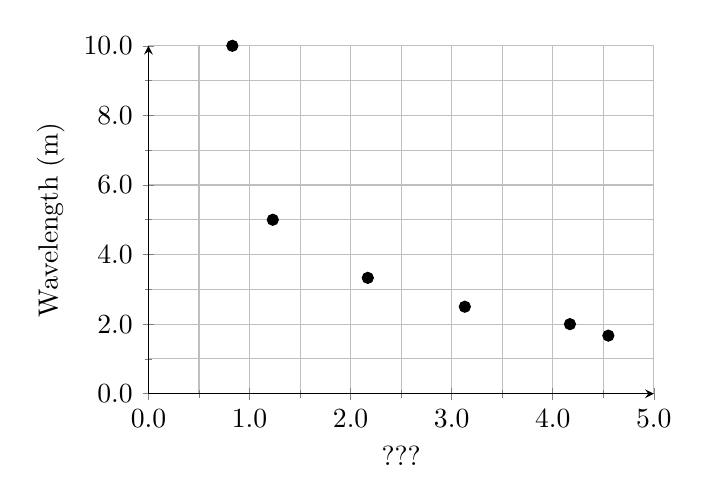
\begin{tikzpicture}
    \begin{axis}[height=6cm,
        width=8cm,
        ylabel={Wavelength (m)},
        xlabel={???},
        axis lines=left,
        ymin=0,ymax=10,
        xmin=0,xmax=5,
        ytick={0,2,...,10},
        xtick={0,1,...,5},
        minor y tick num=1,
        minor x tick num=1,
        grid=both,
        clip=false,
        tick label style={
                /pgf/number format/fixed,
                /pgf/number format/fixed zerofill,
                /pgf/number format/precision=1}
        ]
        \addplot[only marks] coordinates{(0.83,10)(1.23,5)(2.17,3.33)(3.13,2.5)(4.17,2)(4.55,1.67)};
    \end{axis}
\end{tikzpicture}
\end{center}

After forgetting to label the $x$-axis, the teacher deducts 10\% of their grade. Which of the following quantities and units could be plotted on the horizontal axis to produce the inverse relationship?

\ifprintanswers
{\color{red}
$v = f \lambda \quad \Rightarrow \quad \lambda = \frac{v}{f}$, where $v$ is constant for each measurement.
}
\fi

\begin{randomizechoices}
    \correctchoice Frequency (Hz)
    \choice Period (s)
    \choice Wave Speed (m/s)
    \choice Amplitude (m)
\end{randomizechoices}

\clearpage

\question
The Undertaker is a wrestler whose entrance song begins with the ominous chiming of a church bell. Eight chimes are heard in the first 40 seconds of his song. Calculate the frequency of those chimes. 

\ifprintanswers
{\color{red}

$f = \frac{\text{\# cycles}}{\text{total time}} = \frac{\SI{8}{cycles}}{\SI{40}{s}} = \boxed{\SI{0.2}{Hz}}$

\medskip
}
\fi


\begin{randomizechoices}
    \correctchoice \SI{0.2}{Hz}
    \choice \SI{5}{Hz}
    \choice \SI{320}{Hz}
    \choice \SI{0.8}{Hz}
\end{randomizechoices}

\question
A metronome emits clicks at a rate of \SI{4.0}{Hz}. Calculate period between clicks. 

\ifprintanswers
{\color{red}
$T = \frac{1}{f} = \frac{1}{\SI{4.0}{Hz}} = \boxed{\SI{0.25}{s}}$

\medskip
}
\fi

\begin{randomizechoices}
    \correctchoice \SI{0.25}{s}
    \choice \SI{4.0}{s}
    \choice \SI{0.50}{s}
    \choice \SI{8.0}{s}
\end{randomizechoices}

\question
A hummingbird flaps its wings at a high rate of \SI{50}{Hz}. What is the period of oscillation?

\ifprintanswers
{\color{red}
$f = \frac{1}{T} = \frac{1}{\SI{50}{Hz}} = \boxed{\SI{0.02}{s}}$

\medskip
}
\fi

\begin{randomizechoices}
    \correctchoice \SI{0.02}{s}
    \choice \SI{0.05}{s}
    \choice \SI{50}{s}
    \choice \SI{20}{s}
\end{randomizechoices}







\ifprintanswers \else \clearpage \fi

\begin{EnvUplevel}
\textbf{Questions \ref{Q3}--\ref{Q4}.} A rope made of lots of beads is attached to an oscillating machine that produces steady transverse waves across the rope. A student places the other end of the rope near a window to facilitate the counting of wave cycles.

\begin{center}
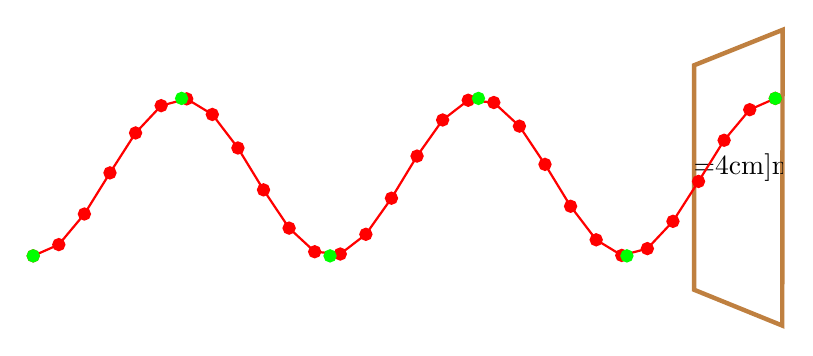
\begin{tikzpicture}
    \begin{scope}[shift={(7.45,-1.43)},x=5mm,y=5mm]]
    \draw[ultra thick,brown] (0,0) -- (0,5.7) -- (2.25,6.6) -- (2.24,-0.91) -- cycle;
    \clip (0,0) -- (0,5.7) -- (2.25,6.6) -- (2.24,-0.91) -- cycle;
    \node at (2,3.1) {\twemoji[height=4cm]{national park}};
    \end{scope}
    \draw[x=6mm,y=1cm,domain=-pi/2:pi/2+4*pi,samples=30,thick,red,mark=*] plot (\x,{sin(\x r)});
    \draw[x=6mm,y=1cm,domain=-pi/2:pi/2+4*pi,samples=6,thick,green,mark=*,only marks] plot (\x,{sin(\x r)});
    % % \draw[<-,very thick] (2.75*pi,1) -- ++(1,0) node[right] {crest};
\end{tikzpicture}
\end{center}
\vspace{-1em}
\end{EnvUplevel}

\question \label{Q3}
What is the number of waves on the string shown in the figure?

\begin{randomizechoices}
    \correctchoice 2.5
    \choice 3.0
    \choice 3.5
    \choice 4.0
\end{randomizechoices}

\question 
Using a stop watch, a student measures the amount of time it takes for 10 full wave cycles to propagate through the window frame. Then, using Desmos, they calculate 10 cycles divided by the total measured time. This calculation determines the wave's

\begin{randomizeoneparchoices}
    \correctchoice frequency
    \choice wavelength
    \choice speed
    \choice period
\end{randomizeoneparchoices}

\question \label{Q4}
The student doubles the oscillation frequency and notes that the wavelength reduces to half the original value. What happened to the wave speed?

\begin{randomizechoices}[norandomize]
    \correctchoice The wave speed stayed constant.
    \choice The wave speed doubled.
    \choice The wave speed was halved.
    \choice There is not enough information. 
\end{randomizechoices}


\bigskip

\hrule

\question
When an ambulance is at rest, it emits a siren at a frequency of $f_0$ corresponding to the rest pitch. The ambulance then moves at speed $v_0$ relative to Alice and Bob, as shown in the figure below. 

\begin{center}
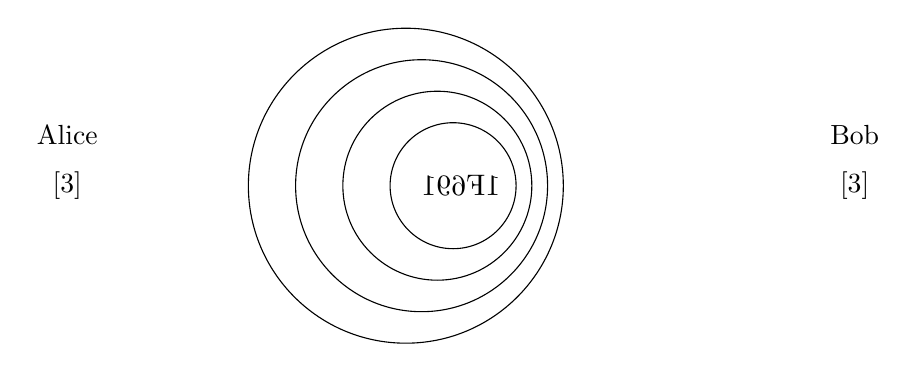
\begin{tikzpicture}
    \draw (-5,0) node {\Strichmaxerl[3]} node[above=4mm] {Alice};
    \draw (+5,0) node {\Strichmaxerl[3]} node[above=4mm] {Bob};
    \node at (0,0) {\reflectbox{\resizebox{1cm}{!}{\usym{1F691}}}}; 
    \draw (-0.10,0) circle (0.8);
    \draw (-0.30,0) circle (1.2);
    \draw (-0.50,0) circle (1.6);
    \draw (-0.70,0) circle (2.0);
\end{tikzpicture}
\end{center}

Alice will hear a pitch that is \fillin[lower than][4cm] the rest pitch, and Bob will hear a pitch that is \fillin[higher than][4cm] the rest pitch.

\begin{randomizechoices}
    \correctchoice lower than; \hspace{1pt} higher than
    \choice higher than; \hspace{1pt} lower than
    \choice lower than; \hspace{1pt} equal to
    \choice equal to; \hspace{1pt} higher than
\end{randomizechoices}

\ifprintanswers \else \clearpage \fi


\question
A rope is attached to a wave and the standing wave shown below is produced.

\begin{center}
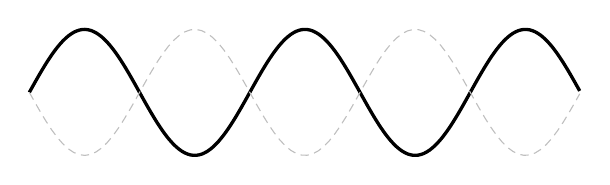
\begin{tikzpicture}[y=8mm,x=7cm]
    \draw[very thick,domain=0:1,samples=100,smooth] plot(\x,{sin(deg(2*pi*2.5*\x))});
    \draw[domain=0:1,samples=100,densely dashed,black!25] plot(\x,{-sin(deg(2*pi*2.5*\x))});
\end{tikzpicture}
\end{center}

How many nodes and antinodes are shown in the figure?

\begin{randomizechoices}
    \correctchoice 6 nodes, 5 antinodes
    \choice 5 nodes, 6 antinodes
    \choice 2.5 nodes, 3 antinodes
    \choice 3 nodes, 2.5 antinodes
\end{randomizechoices}

\question
An incident pulse moving to the right approaches a fixed end.

\begin{center}
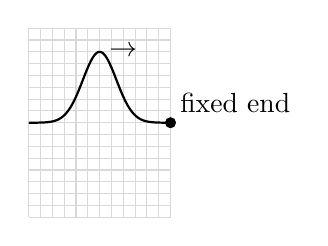
\begin{tikzpicture}[y=3mm,x=3mm]
    \draw[step=0.5,black!15] (0,-4) grid (6,4);
    \draw[domain=0:6,samples=120,thick] plot (\x,{3*exp(-(\x-3)^2)});
    \node[right] at (3,3) {$\rightarrow$};
    \fill (6,0) circle (2pt) node[above right] {fixed end};
\end{tikzpicture}
\end{center}

Which of the following figures represents the reflected pulse?

\begin{center}
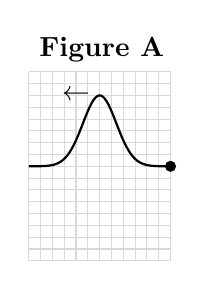
\begin{tikzpicture}[y=3mm,x=3mm]
    \draw[step=0.5,black!15] (0,-4) grid (6,4);
    \draw[domain=0:6,samples=120,thick] plot (\x,{3*exp(-(\x-3)^2)});
    \node[left] at (3,3) {$\leftarrow$};
    \fill (6,0) circle (2pt);
    \node[above] at (current bounding box.north) {\textbf{Figure A}};
\end{tikzpicture}
\hspace{5mm}
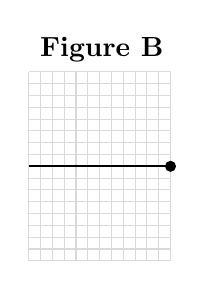
\begin{tikzpicture}[y=3mm,x=3mm]
    \draw[step=0.5,black!15] (0,-4) grid (6,4);
    \draw[domain=0:6,thick] plot (\x,0);
    % \node[left] at (3,3) {$\leftarrow$};
    \fill (6,0) circle (2pt);
    \node[above] at (current bounding box.north) {\textbf{Figure B}};
\end{tikzpicture}
\hspace{5mm}
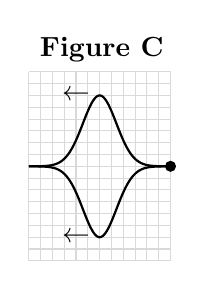
\begin{tikzpicture}[y=3mm,x=3mm]
    \draw[step=0.5,black!15] (0,-4) grid (6,4);
    \draw[domain=0:6,samples=120,thick] plot (\x,{+3*exp(-(\x-3)^2)});
    \draw[domain=0:6,samples=120,thick] plot (\x,{-3*exp(-(\x-3)^2)});
    \node[left] at (3,-3) {$\leftarrow$};
    \node[left] at (3,+3) {$\leftarrow$};
    \fill (6,0) circle (2pt);
    \node[above] at (current bounding box.north) {\textbf{Figure C}};
\end{tikzpicture}
\hspace{5mm}
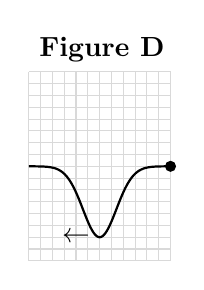
\begin{tikzpicture}[y=3mm,x=3mm]
    \draw[step=0.5,black!15] (0,-4) grid (6,4);
    \draw[domain=0:6,samples=120,thick] plot (\x,{-3*exp(-(\x-3)^2)});
    \node[left] at (3,-3) {$\leftarrow$};
    \fill (6,0) circle (2pt);
    \node[above] at (current bounding box.north) {\textbf{Figure D}};
\end{tikzpicture}
\end{center}

\begin{randomizeoneparchoices}[norandomize]
    \choice Figure A
    \choice Figure B
    \choice Figure C
    \correctchoice Figure D
\end{randomizeoneparchoices}

\question
How do the pitch and amplitude of a sound wave produced by a meowing kitten compare to sound produced by a blue whale?

\begin{randomizechoices}
    \correctchoice The kitten's sound has a higher pitch but smaller amplitude.
    \choice The kitten's sound has a lower pitch but greater amplitude.
    \choice The kitten's sound has a higher pitch and greater amplitude.
    \choice The kitten's sound has a lower pitch and smaller amplitude.
\end{randomizechoices}



\question
The energy of a sound wave is most closely related to its

\begin{randomizechoices}
    \correctchoice amplitude
    \choice period
    \choice frequency
    \choice wavelength
\end{randomizechoices}

% \question
% A long rope is made by connecting a smaller metallic rope to a rubber one. A group of students generate a transverse pulse by distributing one end of the rope.  In Trial one, the pulse is incident along the metal portion, and in Trial 2 the incident pulse travels along the rubber portion, as shown below.

% \begin{EnvUplevel}
% \begin{center}
% \begin{tikzpicture}[y=3mm,x=5mm]
%     \draw[ultra thick,domain=-6:0,samples=120] plot (\x,{4*exp(-(\x+3)^2)});
%     \node[above] at (-3,4) {$\rightarrow$};
%     \draw (0,0) -- (6,0) node[below] {rubber};
%     \draw[densely dashed] (0,3) -- (0,-3) node[below] {boundary};
%     \node[above=] at (current bounding box.north) {\textbf{Trial 1}};
%     \node[below] at (-6,0) {metal};
% \end{tikzpicture}
% \hspace{1cm}
% \begin{tikzpicture}[y=3mm,x=5mm]
%     \draw[domain=-6:0,samples=120] plot (\x,{4*exp(-(\x+3)^2)});
%     \node[above] at (-3,4) {$\rightarrow$};
%     \draw[ultra thick] (0,0) -- (6,0) node[below] {metal};
%     \draw[densely dashed] (0,3) -- (0,-3) node[below] {boundary};
%     \node[above] at (current bounding box.north) {\textbf{Trial 2}};
%     \node[below] at (-6,0) {rubber};
% \end{tikzpicture}
% \end{center} 
% \end{EnvUplevel}

% Which trial will produce a reflected pulse?

% \begin{randomizechoices}[norandomize]
%     \choice Trial 1
%     \correctchoice Trial 2
%     \choice Both trials
%     \choice Neither trial
% \end{randomizechoices}

\question 
Sound waves cannot carry energy through

\begin{randomizechoices}
    \correctchoice a vacuum
    \choice air
    \choice water
    \choice a mirror
\end{randomizechoices}

\ifprintanswers \else \clearpage \fi

\begin{EnvUplevel}
\textbf{Question \ref{longitudinal-wave}--\ref{transverse-wave}.} The figure below shows two waves.

\begin{center}
\tikzset{declare function={f(\x)=sin(540*\x);}}
\begin{tikzpicture}[y=7mm,x=8mm]
     \draw[thick,domain=0.1:9.5,variable=\x,samples=500] plot
     ({\x-1.1*exp(-(\x-2)*(\x-2))-1.1*exp(-(\x-8)*(\x-8))},{f(\x)});
     \draw[|<->|] (0.6,1.3) -- (6.6,1.3) node[above,pos=0.5] {$\lambda$};
     \node[below=5mm] at (current bounding box.south) {\textbf{Wave 1}};
\end{tikzpicture}
\hspace{1cm}
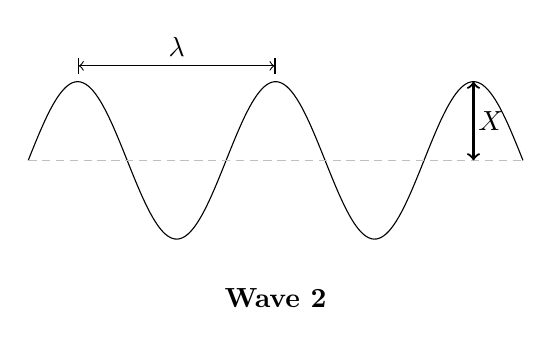
\begin{tikzpicture}[x=4mm,y=1cm]
    \draw[domain=0:2.5*2*pi,samples=200] plot (\x,{sin(\x r)});
    \draw[densely dashed,lightgray] (0,0) -- (2.5*2*pi,0);
    \draw[|<->|] (pi/2,1.2) -- (5*pi/2,1.2) node[above,pos=0.5] {$\lambda$};
    \draw[thick,<->] (9*pi/2,0) -- (9*pi/2,1) node[right=-2pt,pos=0.5] {$X$};
    \node[below=5mm] at (current bounding box.south) {\textbf{Wave 2}};
\end{tikzpicture}
\end{center}

\end{EnvUplevel}

\question \label{longitudinal-wave}
What type of wave is Wave 2?

\begin{randomizechoices}
    \correctchoice transverse wave
    \choice longitudinal wave
    \choice newtonian wave
    \choice seismic wave
\end{randomizechoices}


\question \label{transverse-wave}
What type of wave is Wave 1?

\begin{randomizechoices}
    \choice transverse wave
    \correctchoice longitudinal wave
    \choice newtonian wave
    \choice seismic wave
\end{randomizechoices}


\question
What is the shortest length of an open pipe that resonates at a frequency of \SI{49.0}{Hz} The velocity of sound is \SI{343}{m/s}.

\begin{center}
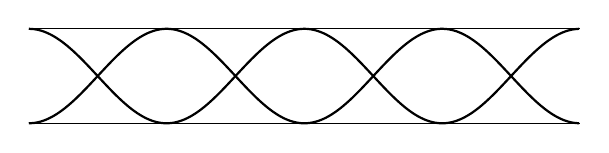
\begin{tikzpicture}[y=6mm,x=7cm]
    \draw (0,1) -- (1,1) (0,-1) -- (1,-1);
    \draw[thick,domain=0:1,samples=100,smooth] plot(\x,{+cos(deg(2*pi*2*\x))});
    \draw[thick,domain=0:1,samples=100,smooth] plot(\x,{-cos(deg(2*pi*2*\x))});
    % \draw[domain=0:1,samples=100,densely dashed,black!25] plot(\x,{-sin(deg(2*pi*2.5*\x))});
\end{tikzpicture}
\end{center}

\ifprintanswers
{\color{red}
$f = \frac{nv}{2L}$, where $n=1$ for shortest pipe, and $v = \SI{343}{m/s}$ is sound speed. $\Rightarrow \quad L = \frac{nv}{2f} = \frac{(1)(\SI{343}{m/s})}{2(\SI{49}{Hz})} = \boxed{\SI{3.5}{m}}$
}
\fi

\begin{randomizechoices}
    \choice \SI{1.75}{m}
    \correctchoice \SI{3.50}{m}
    \choice \SI{14.0}{m}
    \choice \SI{22.0}{m}
\end{randomizechoices}





\end{questions}
\end{document}